\documentclass[12pt,a4paper]{article}
\usepackage[T1]{fontenc}
\usepackage{geometry}
\geometry{tmargin=1in,bmargin=1in,lmargin=1.2in,rmargin=1.2in}
\usepackage[english]{babel}
\usepackage{amsmath}
\usepackage{booktabs}
\usepackage{graphicx}
\usepackage{float}
\usepackage{amsmath}
\usepackage{amssymb}
\usepackage{ae,aecompl}
\usepackage[multiple]{footmisc}
\usepackage[hyperfootnotes=false]{hyperref}
\usepackage{bookmark}
\hypersetup{colorlinks=true,citecolor=blue}
\usepackage{amsthm}
\usepackage{MJOARTI}
\usepackage{setspace}
%\onehalfspacing
%\doublespacing
%\usepackage{vmargin}
\usepackage{graphicx}
\usepackage{rotating}
\usepackage{bbold}
\usepackage{lscape}
\usepackage{subfigure}
\usepackage{caption}
\usepackage{hyperref}
%\usepackage{floatrow}
\usepackage{lscape}
\usepackage{ifthen}
\usepackage{url}
\usepackage{blkarray}
\usepackage{multirow}
\usepackage{tabularx}
\usepackage{longtable}
\usepackage{enumerate}
\usepackage{supertabular}
\usepackage{fancyhdr}
\usepackage{epstopdf}
\usepackage{dsfont}
\usepackage{url}
\usepackage{multicol}
\usepackage{titlesec}
\usepackage{eurosym}
\usepackage{arydshln}
\usepackage{natbib}
\usepackage{threeparttable} % for notes below a table
\usepackage{comment}

\newcommand\citeapos[1]{\citeauthor{#1}'s (\citeyear{#1})}
\newtheorem{theorem}{Theorem}
\newtheorem{algorithm}{Algorithm}
\newtheorem{axiom}{Axiom}
\newtheorem{case}{Case}
\newtheorem{claim}{Claim}
\newtheorem{conclusion}{Conclusion}
\newtheorem{assumption}{Assumption}
\newtheorem{hypothesis}{Hypothesis}
\newtheorem{condition}{Condition}
\newtheorem{conjecture}{Conjecture}
\newtheorem{corollary}{Corollary}
\newtheorem{criterion}{Criterion}
\newtheorem{definition}{Definition}
\newtheorem{example}{Example}
\newtheorem{exercise}{Exercise}
\newtheorem{lemma}{Lemma}
\newtheorem{notation}{Notation}
\newtheorem{problem}{Problem}
\newtheorem{proposition}{Proposition}
\newtheorem{remark}{Remark}
\newtheorem{solution}{Solution}
\newtheorem{summary}{Summary}
\newtheorem{class}{Class}
\usepackage{array}
\newcolumntype{k}{>{\centering\arraybackslash}p{2cm}}
\usepackage{longtable}
\usepackage{ltcaption}
\usepackage{multicol}
\usepackage{color}
\usepackage{textcomp}
\definecolor{dark-red}{rgb}{0.6,0,0}
\definecolor{listinggray}{gray}{0.9}
\definecolor{darkgreen}{rgb}{0,0.4,0}
\definecolor{lbcolor}{rgb}{0.9,0.9,0.9}


%\setlength{\absleftindent}{-0.25in} % For Restart
%\setlength{\absrightindent}{-0.25in} % For Restart

%\renewcommand\thesection{\Roman{section}.}
%\renewcommand\thesubsection{\Alph{subsection}.}

\begin{document}
	
	\date{November, 2023}
	
	\title{Replication Report of "Belief Elicitation and Behavioral Incentive Compatibility" by  Danz et al. (2022)}
	\author{
		George Agyeah\thanks{Authors: 
			Brodeur: University of Ottawa and IZA. E-mail: \href{mailto:abrodeur@uottawa.ca}%
			{abrodeur@uottawa.ca}. For each author: List your affiliation(s) and contact information. Indicate who is the corresponding author if multiple authors. For each author: Acknowledge any financial support or conflict of interest. Describe your relationship with the original author(s) if there is a conflict of interest. Examples of conflict of interest include, but are not limited to, being a colleague, collaborator, current or former student, former thesis supervisor or family member. See I4R’s conflict of interest policy here: \url{https://i4replication.org/conflict.html}.} \and 
		Dario Trujano-Ochoa\thanks{University of California Santa Barbara. E-mail: \href{dariotrujanoochoa@ucsb.edu}%
			{dariotrujanoochoa@ucsb.edu}. There were no conflicts of intereste beetween this authors and the results and authors from the original paper. There is no relationship between the original authors of the paper and Dario Trujano-Ochoa.}}
	
	\maketitle
	
	\onehalfspacing
	\begin{abstract}
		
		%Instructions
		%Summarize in few sentences the original study, focusing on the main results in the original abstract in terms of word claim  which you attempt to reproduce or replicate. 
		
		%By main results, please follow the word claim from the Social Science Replication Platform: “Claims can have different structures, here we propose two high-level categories based on the most common structures:
		
		%Causal claim: a claim is causal if it can be summarize using causal language. This language can be characterize by the following structure: “The paper estimates the effect of a variable X on outcome Y for population P, using method M.” For example: “This paper investigates the impact of bicycle provision (X) on secondary school enrollment (Y) among young women in Bihar/India (P), using a Difference in Difference approach (M).”
		
		%Descriptive/predictive claim: a claim is descriptive or predictive if it can be summarize using descriptive or predictive language. language can be characterize by the following structure: “The paper estimates the value of a variable Y (estimated or predicted) for population P under dimensions X (optional) using method M.” For example, “Drawing on a unique Swiss data set (P) and exploiting systematic anomalies in countries’ portfolio investment positions (M), I find that around 8% of the global financial wealth of households is held in tax havens (Y).”
		
		%Provide information, if relevant, on the magnitude and statistical significance of the main results. Then report all your reproduction and replication results. 
		
		%In the event that there are too many robustness tests per claim to report them individually in the Abstract, then report a summary measure such as the fraction of tests that replicates (i.e., statistically significant in the same direction as the original result) for each claim and the average relative size of the tests for each claim (or the average of these measures across the clams if there are also too many claims being reproduced or replicated to report them individually in the Abstract).
		
		%See below definitions: 
		
		%Computational reproducibility: The ability to duplicate the results of a prior study using the same data and procedures as were used by the original investigator. Reproducibility is done using the same computer code, but can be achieved using a different software package.
		
		%Robustness replicability: The ability to duplicate the results of a prior study using the same data but different procedures as were used by the original investigator. Robustness replicability can be done using the raw, intermediate or final data sets used by the original authors.
		
		%Direct replicability: The ability to duplicate the results of a prior study using new data but the same procedures as were used by the original investigator.
		
		%Conceptual replicability: The ability to duplicate the results of a prior study using new data and different procedures as were used by the original investigator.
		
		\small{
			% summary of the results from the original paper
			In the original paper, \cite{analyst_2022} . 
			%Summary of our findings
			%First, we reproduce the paper’s main findings and uncover two minor coding errors which have no effect on the studies’ main results. Second, we test the robustness of the results to (1) adding more years to the sample and (2) changing how standard errors are clustered. 
			% extended findings
			%We find that adding more years to the sample decreases the size of the point estimate by one-third for education and by one-fourth for fertility. The point estimate for fertility becomes statistically insignificant at the 10\% level, while it remains significant at the 5\% level for education. Clustering at the region level makes the point estimates for education and fertility to be statistically insignificant at the 10% level. 
			
			%
			Example for a direct replication of an experimental study: We conduct a direct replication of the paper by using the same procedures (i.e., method and analysis) and new data. We confirm the sign, magnitude and statistical significance of the point estimates for outcome X.} \newline
		
		
		\textsc{Keywords}:  \newline
		
		\textsc{JEL codes}: .
	\end{abstract}
	
	\clearpage
	\doublespacing
	
	\section{Introduction}
	
	%Instructions
	
	%Briefly describe the main data sources, method, policy or treatment, time period and population for which the estimates apply. Then describe the main scientific claims (descriptive or causal) and robustness checks if those that are relevant for your re-analysis or replication. Quote the original part of the study that has the main scientific claim(s) including page number(s). As suggested in the Guide for Accelerating Computational Reproducibility in the Social Sciences (https://bitss.github.io/ACRE/), structure your summary of the main findings and methodology as follows: "The paper tested the effect of X on Y for population P, using method M. The main results show an effect of magnitude E (specify units and standard errors)" or "The paper estimated the value of Y (estimated or predicted) for population P under dimensions X using method M. The main results presented an estimate of magnitude E (specify units and standard errors)". This template assumes that the paper’s scientific claims are focused on estimating a causal relationship. In the event that the original study is estimating/predicting a descriptive statistic of a population, or something else, then describe and quote the results accordingly using precise claims from the original study.
	
	%How to select claims to reproduce/replicate? There are three possibilities; (1) select claims for all "hypotheses tests" in the original study, (2) select claims mentioned in the abstract or (3) select claims for what is considered the main result in the paper as stated by the original author(s). For the last option, provide a quote from the original study confirming that the claim chosen is considered the main result by the original author(s).       	
	
	%Next, summarize your reproduction and/or replication. Start by stating how you have obtained the data and codes and if the original author(s) answered your request(s) a/nd questions. Indicate the repository where your programs and data are located. Then proceed with a description of your conceptual reproducibility by describing if you have found coding error(s) and how they affect the main conclusions.
	
	%For replication, we adopt the definitions here. For robustness replicability, clearly state your robustness checks and how they affect the main point estimates. For direct and conceptual replications, clearly describe the new data. For conceptual replications, also describe the new procedures or they differ from the original study. Different procedures implies a different experimental design and/or analysis for experiments and different methods and/or analysis for observational data.
	
	%For all three replication types, be precise and summarize your results as follows: “Implementing this robustness increases/decreases the size of the main point estimate for outcome Y by X and the estimate is not anymore statistically significant at the X% level ” or "Implementing this robustness check has no effect on the magnitude or the statistical significance of the main point estimate." Also report the coefficient (or other effect size), the standard error of the coefficient/effect size, the test statistic including df if relevant, and the p-value for all tests.
	
	\textbf{Example:} 
	%(see above for instructions)%
	
	\cite{analyst_2022}, henceforth DVW, 
	
	
	\section{Reproducibility}
	
	During our investigation, we noticed that the frequency of the priors is not balanced, as shown in table \ref{priors} below. Specifically, each individual is randomly assigned priors with a 0.5 probability four times as often as prior 0.2 and prior of 0.8 independently. Similarly, priors of 0.3 and 0.7 are assigned twice as many times as priors of 0.2 and 0.8 independently. We are curious whether the lower false report rates in figure 2b specific to prior belief of 0.5 are a result of learning given the repetition of priors. It is possible for participants to get a better understanding of the optimal strategy as they proceed in the experiment. Hence, priors with lower frequencies should exhibit a different distribution compared to priors that are shown multiple times.
	
	\begin{table}[H]
		\centering
		\caption{Number of pbservations in each treatment by prior} \label{tab:table1}
		\begin{threeparttable}
			\footnotesize 
			{
	\def\sym#1{\ifmmode^{#1}\else\(^{#1}\)\fi}
	\begin{tabular}{l*{1}{ccccccc}}
		\toprule
		Prior & Info & RCL & No Info  & Feedback(t=1,2) & Feedback(t=9,10) & Description   \\
		\midrule
		20         &      120 &         59 &      120   &      8  &   16  &  60 \\
		\midrule
		30         &      240 &        118 &      240   &      21  &   22 &  120 \\
		\midrule
		50         &      480 &        236 &      480   &      55  &   51 &  240 \\
		\midrule
		70         &      240 &        118 &      240   &      24  &   21 &  120 \\
		\midrule
		80         &      120 &         59 &      120   &      12  &   10 &  60 \\
		\bottomrule
	\end{tabular}
} 
			\begin{tablenotes}
				\scriptsize 
				\item{Notes: The priors of participants differed by number of observations.
				}
			\end{tablenotes}  
		\end{threeparttable}                          
	\end{table} \label{priors}
	
	
	\hspace *{0mm} Specifically, if there is learning involved, the rate of false reports for priors with single frequencies will be random across periods since a participant is assigned a prior randomly. On the contrary, the priors with multiple frequencies will see a gradual decrease in the false report rates as the games proceed. If an individual learns each time he/she is presented with the same scenario, then as the individual continues to get more exposure to prior 0.5 relative to the other priors, he/she will get better at giving answers regarding that prior, leading to a similar distribution in figure 2b in the paper.
	
	\hspace *{0mm} In order to further understand the effect of learning or the lack of it, we replicate figure 2a for each prior for only the information treatment. Our hypothesis in this investigation is that considering some priors have a higher frequency than others, there will be some heterogeneous distributions of the distributions of each prior over periods. Let's consider a scenario prior where participants encounter 0.5 four times. If there is learning among the participants causing them to reduce the false report rate, then the error rate for the priors of 0.5 will have an inverse relationship with periods. In contrast, for example, prior 0.2, prior 0.5 should look different. As a matter of fact, given the random assignment of the priors, there should not be a visible trend as the game proceeds if there is no learning. We present the result of these analyses below.
	
	\section{Replication}
	
	%Instructions
	
	%Clearly state/describe which type of replication you are conducting. See definitions at the beginning of this document. For robustness replicability, present your robustness checks and how they impact the main point estimates one by one so that it is clear how each modification to the specification/analysis impacts the main conclusions. Then you may combine them. Also, clearly state why you conduct each specific robustness check and/or modify the setting/model.
	
	%Do not confuse general critiques of the original research with replication or robustness checks (\cite{brown2018tests}). For instance, any critique of the design or methodology (e.g., qualitatively discussing the validity of an exclusion restriction for an instrumental variable) should be included in a separate section and clearly labeled as general critiques rather than a replication exercise.
	
	% \textbf{Example:} 
	%(see above for instructions)%
	
	\subsection{George}
	First, we present figure A, a replication of figure 2a in the original paper in the R programming language. As shown in figure A below, there is no trend as the game proceeds. Next, we present figure B. Figure B shows the Fraction of False Reports conditional on the prior probability being 0.2. Besides the lack of an obvious trend, the intervals for the prior of 0.2 are wide due to the low number of counts relative to other priors. The nature of the confidence intervals is similar to the priors of 0.8 in figure F, which, like 0.2, is shown 1 time to a participant.
	
	\hspace *{0mm} Next, we look at the results of figures C and E together. Figure C shows the fraction of false reports conditioned on the prior probability being 0.2, and Figure E shows the fraction of false reports conditioned on the prior probability being 0.7. It is important to highlight that both priors – 0.3 and 0.7 occur randomly 2 times per participant. First, the range of the error bars reduces relative to those seen in figures A and F discussed above. Secondly, there is no trend in the false report rates across. In fact, errors increase beyond period 5 for prior 0.3 (Figure C), where it is more likely that participants have already been presented with the scenario.
	
	\hspace *{0mm} Finally, we present the results of figure D. If there is learning conditional on the number of times a participant has experienced a scenario, it should be more obvious in this figure. Across the information treatment, each participant experiences the prior probability of 0.5 four times – 2 times as often as priors 0.7 and 0.3 and 4 times as often as priors 0.8 and 0.2. First, it is observed that the range of the error bars is lower as compared to the other priors due to the higher frequencies across rounds. Additionally, there is a trend before the midpoint of the game and after the midpoint. Before period 5, it is observed that the point false reports decrease as the game progresses. This is consistent with learning. However, the trend switches after period 5 where errors tend to increase with each additional period. Under the assumption that a larger portion of people seeing the prior of 0.5 at period 6 have experienced it compared to the participants seeing the same prior probability at period 5, there should be a lower false report, not higher as observed in figure D. This shows the learning observed in the first 5 periods is not consistent in the next 5 periods. 
	
	\subsection{Dario}
	
	
	
	\subsection{Regression model}
	
	
	
	\subsection{Results educational attainment}
	
	\subsubsection{Extending the time period}
	
	
	\subsubsection{Clustering}
	
	
	\section{Conclusion}
	
	%Instructions
	%State the most important results of your work and what you have learned. You may also describe other empirical exercises that could be conducted by other replicators.
	
	
	
	\newpage
	\bibliographystyle{kluwer}
	\bibliography{biblio}
	
	\newpage
	\section{Figures}
	
	\begin{figure}
		\centering
		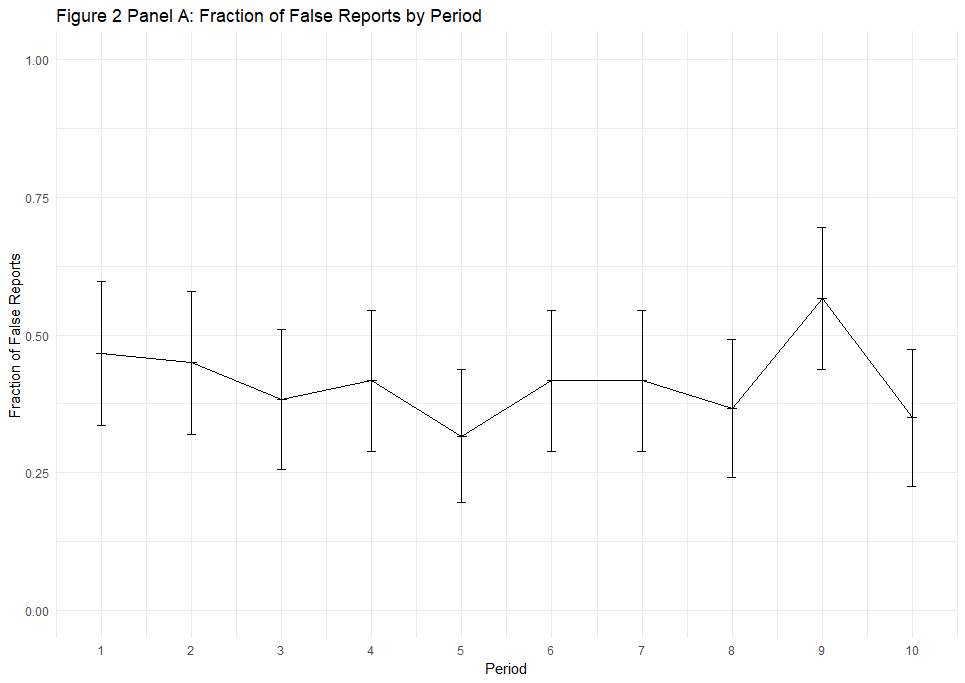
\includegraphics[scale=0.4]{../../results/2a_rep.png}
		\caption{Fraction of False Reports by Period} \label{tab:R1}
		\label{fig:enter-label}
	\end{figure}
	
	\begin{figure}
		\centering
		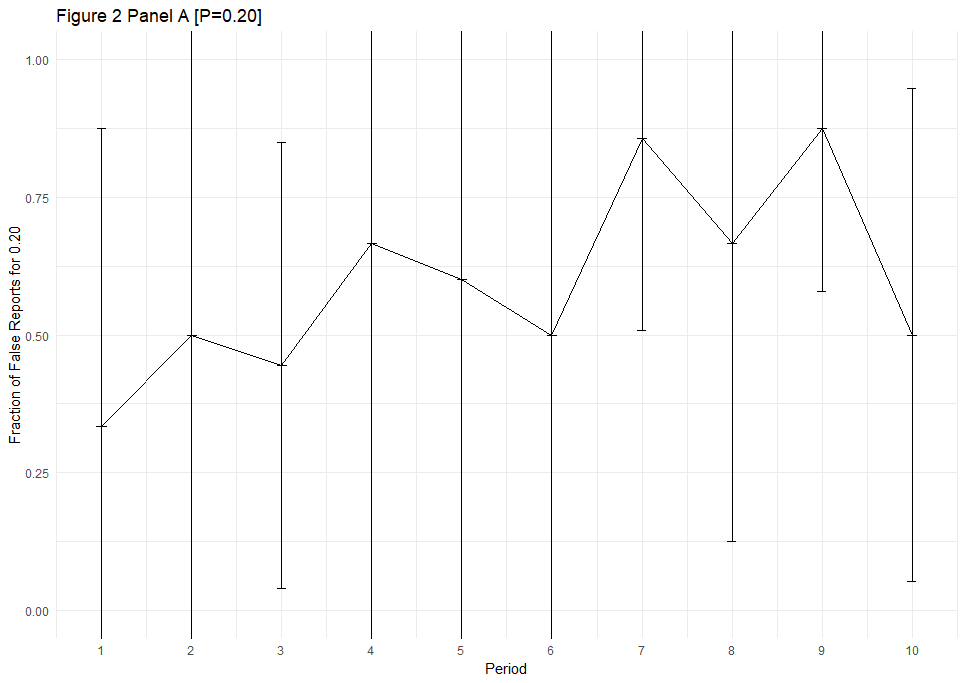
\includegraphics[scale=0.4]{../../results/2a_20.png}
		\caption{Fraction of False Reports by Period Conditional on Prior Probability of 0.2} \label{tab:F2}
		\label{fig:enter-label}
	\end{figure}
	
	\begin{figure}
		\centering
		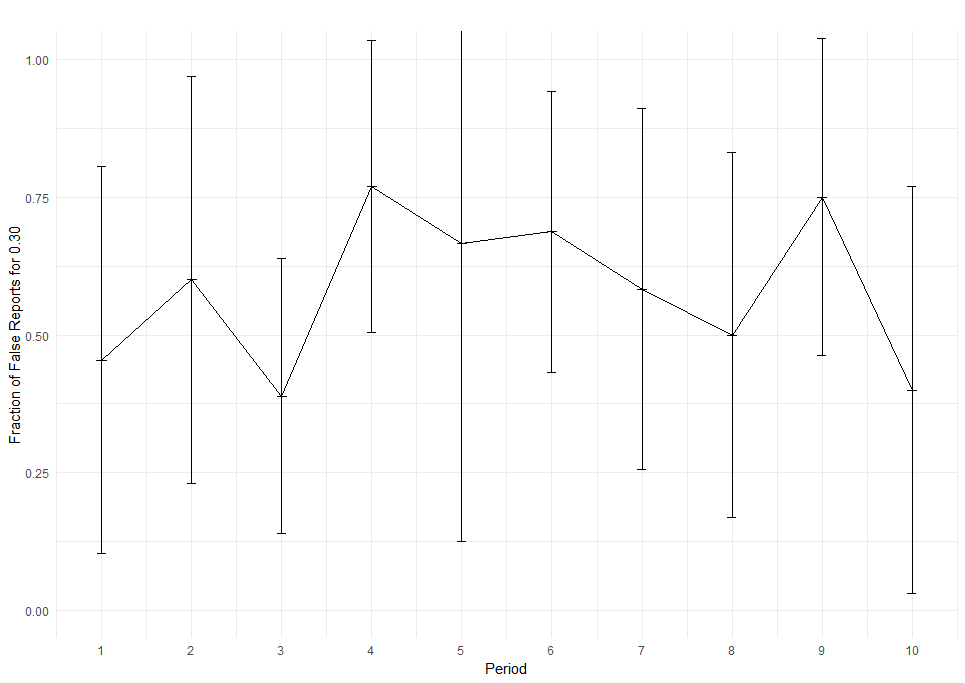
\includegraphics[scale=0.4]{../../results/2a_30.png}
		\caption{Fraction of False Reports by Period Conditional on Prior Probability of 0.3} \label{tab:F3}
		\label{fig:enter-label}
	\end{figure}
	
	\begin{figure}
		\centering
		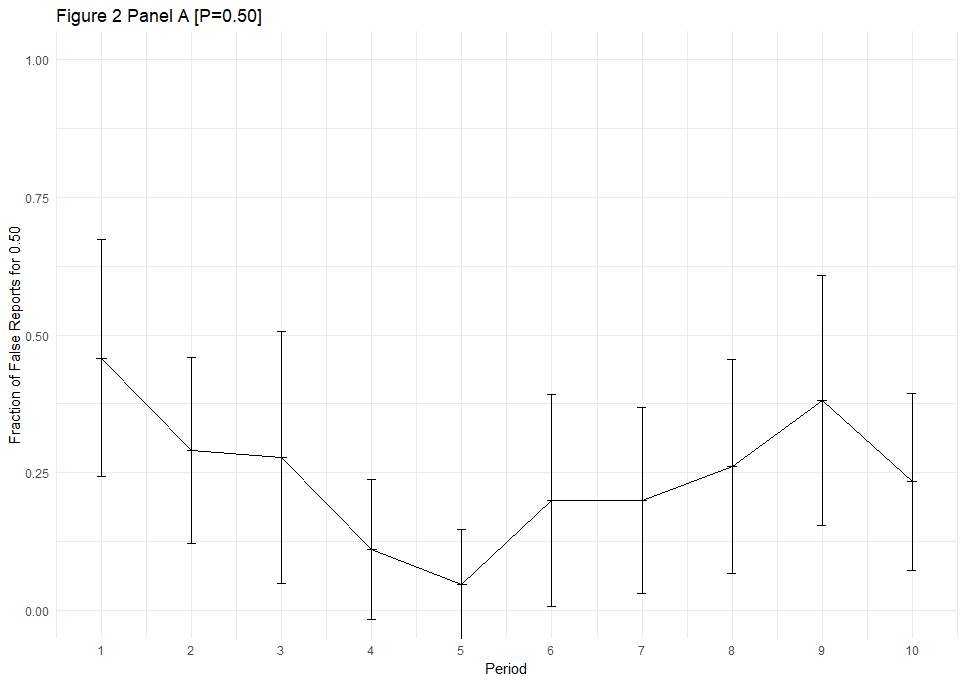
\includegraphics[scale=0.4]{../../results/2a_50.png}
		\caption{Fraction of False Reports by Period Conditional on Prior Probability of 0.5} \label{tab:F4}
		\label{fig:enter-label}
	\end{figure}
	
	\begin{figure}
		\centering
		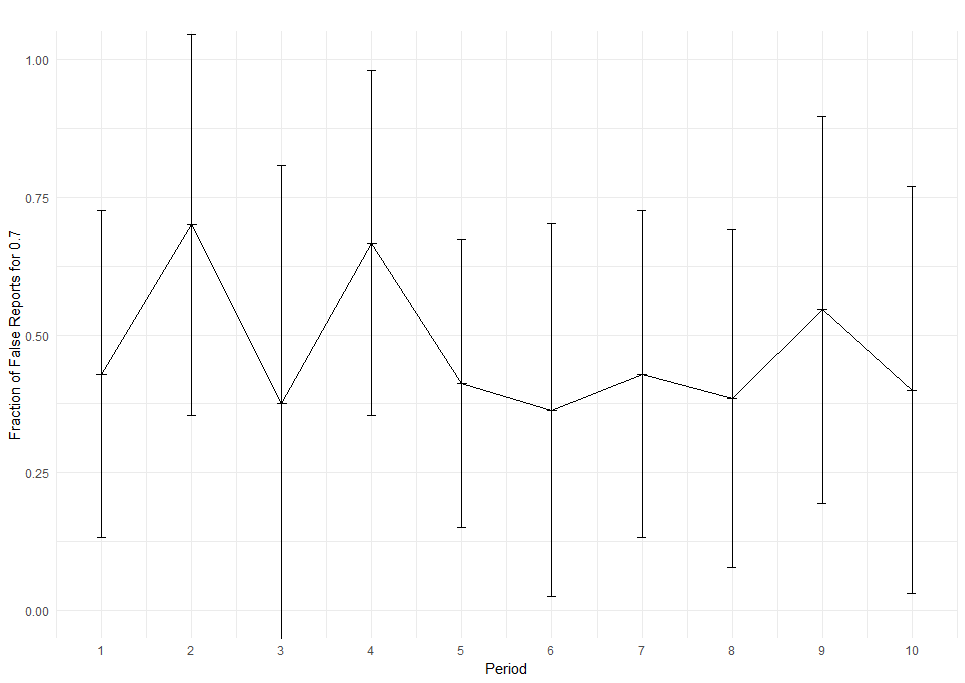
\includegraphics[scale=0.4]{../../results/2a_70.png}
		\caption{Fraction of False Reports by Period Conditional on Prior Probability of 0.7} \label{tab:F5}
		\label{fig:enter-label}
	\end{figure}
	
	\begin{figure}
		\centering
		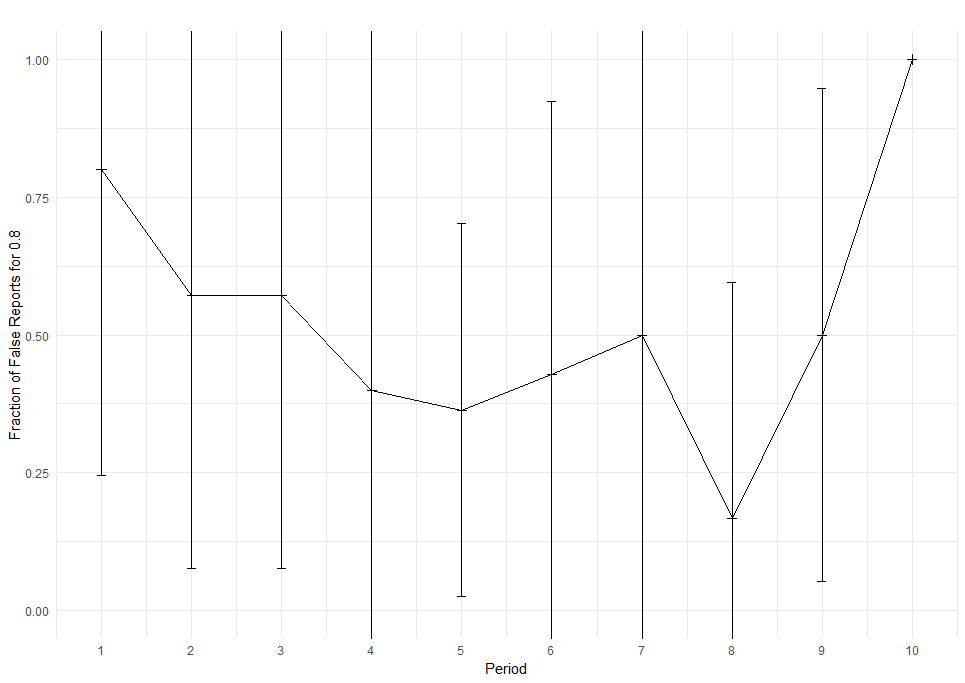
\includegraphics[scale=0.4]{../../results/2a_80.png}
		\caption{Fraction of False Reports by Period Conditional on Prior Probability of 0.8} \label{tab:F6}
		\label{fig:enter-label}
	\end{figure}
	
	
	\newpage
	
	\begin{figure}
		\centering
		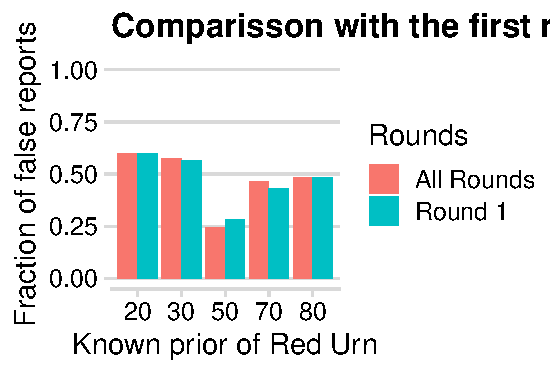
\includegraphics[scale=0.75]{../../results/fig2B_round_one.pdf}
		\caption{Comparisson of the fraction of false reports between all rounds and only the first one by prior. Notice that, in this comparisson, the knowm priors 20 and 80 only have one round and therefore they are the same.}
		\label{fig:fig2a_rounds}
	\end{figure}

	\begin{figure}
	\centering
	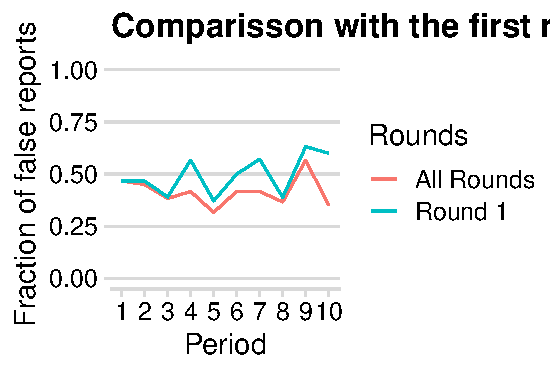
\includegraphics[scale=0.75]{../../results/fig2A_round_one.pdf}
	\caption{Comparisson of the fraction of false reports between all rounds and only the first one by period.}
	\label{fig:fig2b_rounds}
	\end{figure}
	
	\begin{figure}
		\centering
		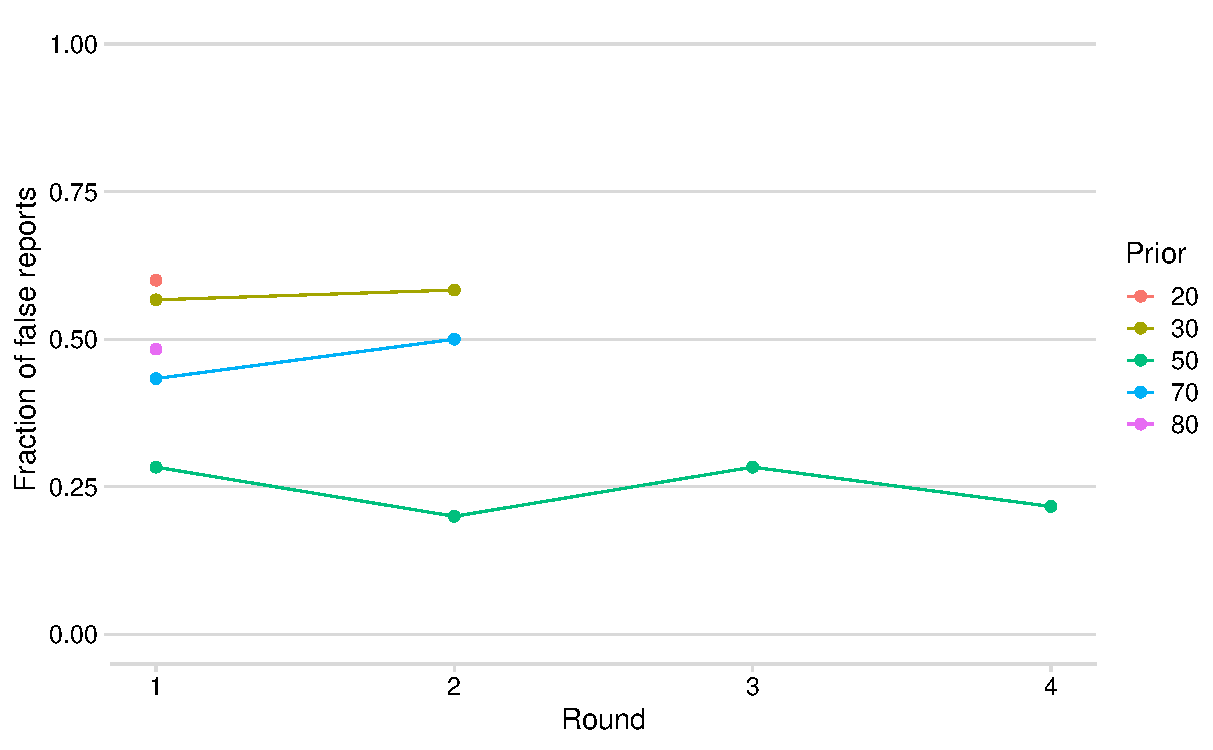
\includegraphics[scale=0.75]{../../results/rounds_all_priors.pdf}
		\caption{Comparisson of the fraction of false reports between priors by round. Each round is the relative position of the prior being presented among the ten periods.}
		\label{fig:rounds_priors}
	\end{figure}

	\begin{figure}
		\centering
		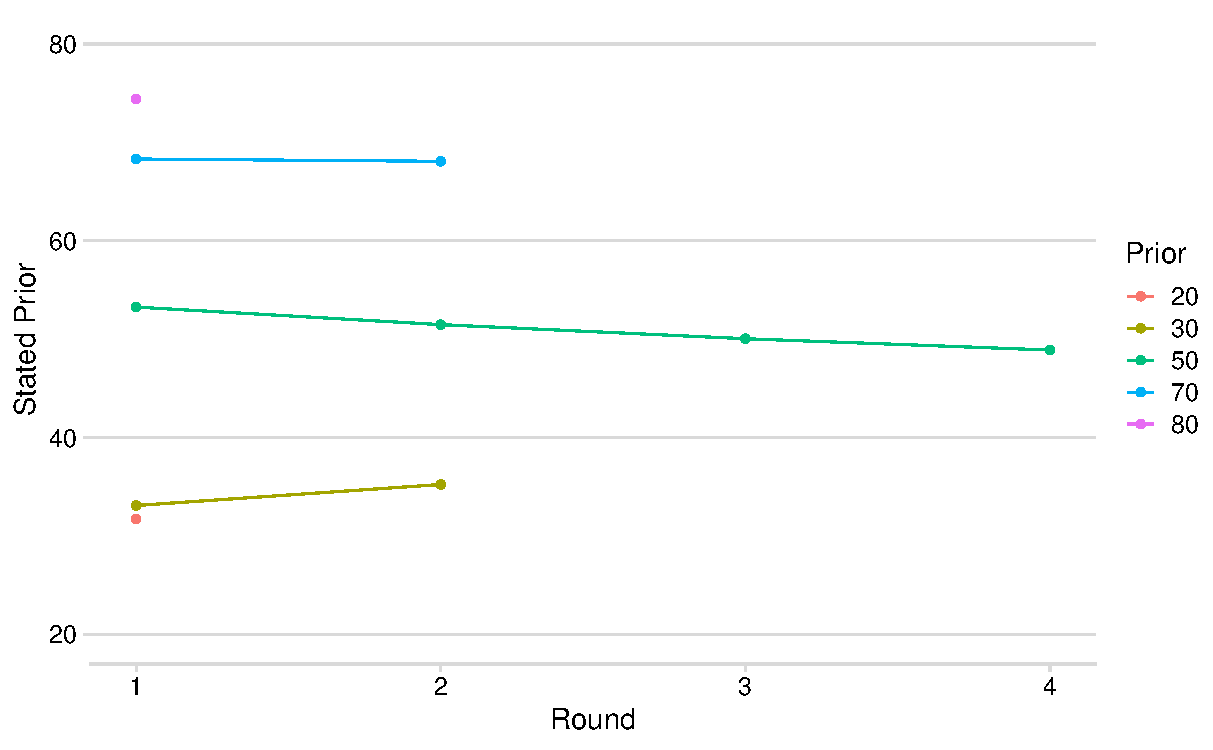
\includegraphics[scale=0.75]{../../results/rounds_stated_prior.pdf}
		\caption{Comparisson of the stated prior between indicated priors by round. Each round is the relative position of the prior being presented among the ten periods.}
		\label{fig:rounds_stated_priors}
	\end{figure}


\end{document} 